\section{Results} \label{sec:results}
% 1. Accuracy (F1 + MCC) auf SICK und eSNLI einzeln nach Kategorien
% 2. Auf Bias überprüfen: Vergleich vom Modell für wichtig erachtete Token mit von Menschen als wichitg erachtete Tokens
% Visualisierungen:
% - Confusion Matrix (Gentrennt nach Phänomenen)
% - Tabellen Interpretability Metriken (siehe ferret)

To analyze the performance of the \acp{LM}, we test their predictive performance and their bias. We provide different scores and visualizations to test our hypothesis and provide insights into the datasets and \acp{LM}.
% Accuracy

To measure the predictive performance, we provide the macro $\text{F}_1$-score \cite{macrof1} and \ac{MCC} \cite{mcc}, as \ac{MCC} has proven to be more reliable than accuracy and $\text{F}_1$ \cite{mccGood}.

% Bias
\paragraph{Bias detection}
To analyze biases, we compare the words deemed important by the \ac{e-SNLI} explanations to the tokens deemed important for the model prediction by interpretability methods. Furthermore, to detect linguistic biases, we conduct a confusion analysis for each specific linguistic phenomenon.

\begin{figure}[ht]
    \centering
    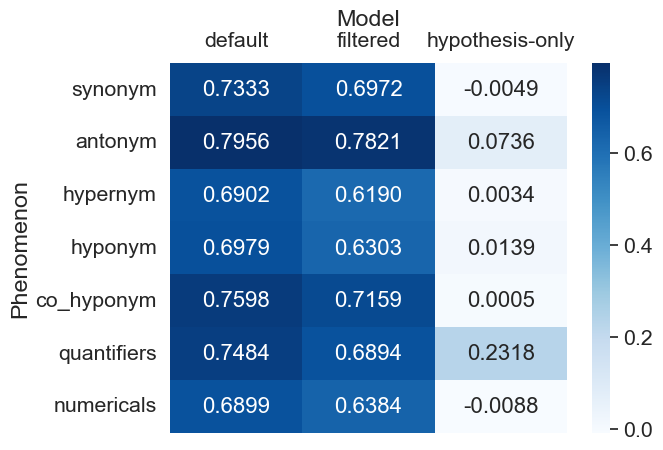
\includegraphics[width=0.9\columnwidth]{./images/metric_heatmaps_phenomena/important_words/matthews_correlation.png}
    \caption{Matthews Correlation Coefficients for the model trained on different datasets on linguistic phenomena}
    \label{fig:metric-heatmap-phenomena-mcc}
\end{figure}

Figure~\ref{fig:metric-heatmap-phenomena-mcc} depicts the Matthews Correlation Coefficients for our model trained on different datasets on different linguistic phenomena: \enquote{default} is the model trained on the regular \ac{MultiNLI} dataset, \enquote{filtered} trained on samples which where correctly classified of maximum two hypothsis only models and \enquote{hypothesis-only} is the model trained only on the hypotheses of \ac{MultiNLI}.

I can be seen that the default model performs best on samples which contain antonyms. The hypothesis-only model performes poorly as expected but also comparably well on antonyms which indicates a bias in these samples. This is confirmed by the better performance of the filtered model on antonyms.

The hypothesis-only model also performes slightly better on samples which contain quantifiers which indicates a bias also in these samples. The filtered model performes slightly worse on quantifiers than the default model. This behavior is probably caused by a lack of training samples as many of them where filtered out for being biased.

% Ferret
To generate explanations we use the interpretability methods Integrated Gradients \cite{integratedgradients}, \ac{LIME} \cite{lime} and Partition SHAP Values \cite{shap}. We use the plausibility and faithfulness \cite{ferret} metrics to judge the model bias.

To demonstrate the biases, we provide example sentences with important tokens highlighted. Furthermore, to provide a different view on the importance of certain tokens, we visualize the attention maps.